\documentclass[11pt,twoside,a4paper]{article}
%\usepackage[options]{extension}
\usepackage{amssymb}
\usepackage{amsmath}
\usepackage{graphicx}
\usepackage[T1]{fontenc}
\usepackage[english,francais]{babel}

\graphicspath{ {./img/} }
\setlength{\parindent}{0pt}
\author{Adela Patcas}
\title{Signal Spaces}

\begin{document}

\maketitle{Signal Spaces}
% insérer la table des matières
Le langage constitue un puissant filet lâche avec lequel aller à la pêche aux faits simples, alors que les faits sont infinis.

Ce chapitre concerne principalement deux types d'objets mathématiques: les espaces métriques et les espaces vectoriels linéaires. L'idée derrière un espace métrique est 
simplement que nous fournissons un moyen de mesurer la distance entre des objets mathématiques, tels que des ensembles, des points, des fonctions ou des séquences. 
Avec cette notion de distance nous pourrons généraliser certains des concepts familiers du calcul, comme la continuité ou la convergence, au-delà des opérations sur une 
seule dimension vers les opérations dans des dimensions supérieures.

Le concept d'espace vectoriel est également simple: il s'agit d'un ensemble d'objets qui peuvent être combinés entre eux à l'aide de combinaisons linéaires. 
Mais la théorie des espaces vectoriels a des ramifications considérables, couvrant une partie importante de la théorie du traitement du signal. Un élément clé de la 
théorie de l'espace vectoriel est que, dans un sens géométriquement utile, les \textbf{fonctions (c'est-à-dire les signaux) peuvent être considérées comme des vecteurs}. 
Cette compréhension géométrique fournit un outil puissant pour l'analyse du signal. Dans ce chapitre, la théorie de base et la notation des espaces vectoriels sont développées. 
Dans le chapitre 3, nous mettons cette notion en pratique dans diverses applications, notamment le filtrage optimal (moindres carrés et carrés moyens minimaux), les transformations, 
la compression de données, l'échantillonnage et l'interpolation.

Dans notre étude des espaces métriques et des espaces vectoriels, l'intention est de fournir un cadre pour la discussion générale des signaux. Avant de commencer ce chapitre, 
le lecteur est encouragé à revoir les définitions de base des fonctions et des ensembles apparaissant dans l'annexe A. Dans cette étude, la notation matricielle est largement 
utilisée dans les sections, donc la révision des notations matricielles de base présentées dans l'annexe C est également recommandée.

Dans le développement de ce chapitre, nous construisons successivement des \textbf{espaces métriques}, des \textbf{espaces vectoriels}, des \textbf{espaces vectoriels normés}, puis des espaces de \textbf{produits internes normés}. 
Cela nous amènera à l'idée importante des projections et des projections orthogonales. La projection orthogonale sera un outil d'une importance capitale pour nous dans le prochain chapitre, 
où elle sera utilisée comme base géométrique pour le filtrage et la prédiction par les moindres carrés et les carrés moyens minimaux.

\section{Espaces métriques}

Nous pouvons considérer que les signaux (fonctions) qui nous intéressent dans un problème particulier sont membres d'un ensemble $X$. En étudiant et en appliquant ces signaux, nous pouvons être intéressés à comprendre 
comment un signal se compare aux autres signaux de cet ensemble. Une façon d'y parvenir consiste à mesurer une "distance" entre les signaux en utilisant une mesure de distance qui est à la fois mathématiquement significative 
et physiquement significative. Les aspects mathématiques d'une fonction de mesure utile sont exprimés dans la définition suivante.

\vspace{5mm}

\textbf{Définition 2.1} Une \textbf{métrique} $d: X \times X \longrightarrow \mathbb{R}$ est une fonction utilisée pour mesurer la distance entre les éléments d'un ensemble $X$. 
Pour être une métrique, elle doit satisfaire aux propriétés suivantes. pour $x, y \in \textit{X}$:
\vspace{2mm}

M1 $d(x, y) = d(y, x)$.

M2 $d(x, y) \geq 0$.

M3 $d(x, y) = 0$ si et seulement si $x = y$.

M4 Pour tous les points $x, y, z \in \textit{X}$,

\begin{equation}
       d(x, z) \leq d(x, y) + d(y, z).
\end{equation}

\vspace{10mm}

\textbf{Exemple 2.1.1} Pour $x, y \in \mathbb{R}$ nous pouvons définir une métrique en utilisant la fonction valeur absolue par

\begin{equation*}
       d(x, y) = |x - y|.
\end{equation*}

Les propriétés requises d'une métrique sont toutes satisfaites. La dernière propriété découle de \textbf{l'inégalité triangulaire}, 
ainsi appelé en raison de la relation qui s'impose sur les glissières d'un triangle plan. Soit $x$,$y$ et $z$ désignent les coins d'un triangle, 
comme le montre la figure 2.1. Alors $d(x, z)$ est la longueur d'un côté,

%\begin{figure}[h]
%  \centering
%  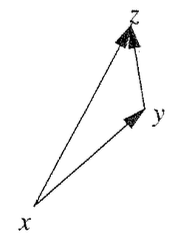
\includegraphics[scale=0.8]{fig2.1}
%  \caption{Illustration de l'inégalité triangulaire}
%\end{figure}

$d(y, z)$ est la longueur du deuxième côté et $d(x, z)$ est la longueur du troisième côté. 
La longueur du le troisième côté ne peut pas être plus long que la longueur des deux premiers côtés.

\vspace{10mm}

Il existe une variété de mesures utilisées; l'exemple suivant en illustre quelques-uns.

% PAGE 73

\textbf{Exemple 2.1.2} Soit $X$ l'ensemble des nombres dans $\mathbb{R}^n$. Soit $x \in \mathbb{R}^n$ et $y \in \mathbb{R}^n$.

\begin{enumerate}
  \item La métrique $d_1:\mathbb{R}^n \times \mathbb{R}^n \longrightarrow \mathbb{R}$ définie par
  
  \begin{equation*}
    d_1(x, y) = \sum_{i=1}^{n} |x_i - y_i|
  \end{equation*}
  
  est appelée métrique $l_1$, également connue sous le nom de métrique de Manhattan, car la distance mesurée dans une ville disposée sur une grille 
  cartésienne doit suivre tout droit le long des rues. La satisfaction de la propriété (2.1) pour cette métrique découle de l'inégalité troangle appliquée à chaque terme.
  \item La métrique $d_2:\mathbb{R}^n \times \mathbb{R}^n \longrightarrow \mathbb{R}$ définie par
  
  \begin{equation*}
    d_2(x, y) = \left({\sum_{i=1}^{n} |x_i - y_i|^2}\right)^{1/2}
  \end{equation*}

  est appelée métrique $l_2$. Il représente la distance euclidienne entre les points. Le fait que cette métrique satisfait la propriété (2.1) est prouvé dans la section 2.6.
  \item En généralisant les deux premières métriques, nous avons
  
  \begin{equation*}
    d_p(x, y) = \left({\sum_{i=1}^{n} |x_i - y_i|^p}\right)^{1/p}
  \end{equation*}

  C'est la métrique $l_p$. Le fait que cette métrique satisfasse (2.1) découle de l'inégalité de Minkowski, qui est démontrée dans l'annexe A.
  \item Comme $p \longrightarrow \infty$, la métrique $l_p$ devient la métrique $l_\infty$,
  
  \begin{equation*}
    d_\infty(x, y) = \max\limits_{i=1,2,...,n} |x_i - y_i|.
  \end{equation*}
\end{enumerate}

\textbf{Exemple 2.1.3} Considérons un vecteur $x \in \mathbb{R}^n$ qui doit être approché (quantifié) par un vecteur comme $\hat{x}$ illustré sur la figure 2.2. 
Pour avoir une bonne représentation des données, nous souhaitons que $\hat{x}$ "ressemble" à x, selon certains critères, et le quantificateur doit être conçu en gardant cela à l'esprit. 
Bien que de nombreuses métriques différentes aient été examinées, les métriques utilisées dans la conception du quantificateur s'avèrent souvent être l'une de celles mentionnées 
ci-dessus, telles que $d_1(x, \hat{x})$ ou $d_2(x, \hat{x})$.

%\begin{figure}[h]
%  \centering
%  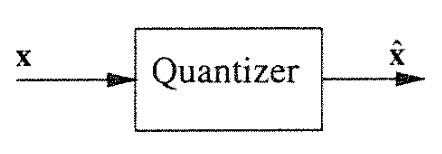
\includegraphics[scale=0.8]{fig2.2}
%  \caption{Quantification du vecteur x}
%\end{figure}

\textbf{Exemple 2.1.4} Soit \textbf{x} une séquence binaire, $\textbf{x} = \{x_0, x_1,...,x_{n-1}\}$, où $x_i$ vaut 0 ou 1. Cette séquence est transmise via un canal où elle peut être 
corrompue par du bruit. La séquence reçue est $\textbf{y} = \{y_0, y_1,...,y_{n-1}\}$. Lors de la réception de telles séquences, l'objectif d'une bonne réception est que les bits de \textbf{y}
correspondent aux bits de \textbf{x}. Une métrique appropriée pour ce critère est la \textit{distance de Hamming} entre les séquences, qui est le nombre de places où $x_i$ et $y_i$ sont différents,

\begin{equation*}
  d_H(x, y) = \sum_{i=0}^{n-1} h(x_i - y_i)
\end{equation*}

où

\begin{equation*}
  h(x, y) = 
\end{equation*}

Lorsque \textbf{x} et \textbf{y} sont des séquences binaires, alors la distance de Hamming qui les sépare peut s'écrire

\begin{equation*}
  d_H(x, y) = \sum_{i=0}^{n-1} x_i \oplus y_i ,
\end{equation*}

dans lequel $\oplus$ désigne l'addition modulo 2.

% PAGE 74

\textbf{Définition 2.2} Un \textbf{espace métrique} $(X, d)$ est un ensemble $X$ avec une métrique $d$.

Il existe de nombreux espaces métriques possibles. Nous commençons par les espaces métriques définis pour les séquences.

\textbf{Exemple 2.1.5}
\begin{enumerate}
  \item L'ensemble $\mathbb{R}^n$ équipé de la métrique $d_2(x, y)$ est un espace métrique.
  \item Soit $l_p = l_p(0, \infty)$ l'ensemble constitué de toutes les séquences infinies de nombres réels ou complexes $\{x_0, x_1,...,x_{n-1}\}$ tels que
  $\sum_{i=0}^{\infty} |x_i|^p < \infty$. Nous prendrons $1 \leq p < \infty$. La fonction
  \begin{equation*}
    d_p(x, y) = \left[{\sum_{i=0}^{\infty} |x_i - y_i|^p}\right]^{1/p}
  \end{equation*}
  définit une métrique sur $l_p$, que nous appellerons la métrique $l_p$. Nous appelons cet espace métrique l'espace $l_p(0, \infty)$, ou simplement l'espace $l_p$. 
  Il s'agit d'un espace de dimension infinie appelé \textit{espace de séquence}.

  L'ensemble des séquences bilatérales $\{...,x_{-1}, x_0, x_1,...\}$ de métrique $d_p$ donne l'espace métrique $l_p(-\infty, \infty)$.

  Dans les applications de traitement du signal en temps discret, nous traitons le plus souvent de l'espace $l_1$ ou de l'espace $l_2$, le premier parce que les valeurs absolues sont faciles à calculer, et le second parce que la fonction métrique quadratique est facilement différentiable.

  \item L'espace $l_\infty(0, \infty)$ est constitué de toutes les suites de nombres $\{x_0, x_1, x_2,...\}$ telles que $|x_n| \leq M$ pour une borne finie $M$ , équipée de la métrique
  
  \begin{equation}
    d_\infty(x, y) = \sup\limits_n |x_n - y_n| .
  \end{equation}
  Voir encadré 2.1. L'espace correspondant des séquences bilatérales est noté $l_\infty(-\infty, \infty)$.
\end{enumerate}

Il existe également de nombreux espaces métriques utiles définis sur les fonctions. Ces espaces de dimension infinie sont appelés \textit{espaces fonctionnels}.

\textbf{\textit{L'espace métrique} $(C[a, b], d_p)$.} Soit $X = C[a, b]$ l'ensemble des fonctions continues à valeurs réelles (ou à valeurs complexes) définies sur l'intervalle $[a, b]$, avec $b > a$. Nous pouvons définir une

% Box 2.1 Sup and inf
\vspace{7mm}
\fbox{%
    \parbox{\textwidth}{%
\textbf{Encadré 2.1: Sup et inf}
}%
}

\fbox{%
    \parbox{\textwidth}{%
Pour un ensemble $S \subset \mathbb{R}$, la moindre limite supérieure (LUB) est le plus petit nombre $z$ tel que $z \geq x$ pour chaque $x \in S$. Le LUB d'un ensemble $S$ est appelé le \textbf{sup} (supremum) de l'ensemble. S'il n'y a pas de nombre supérieur à tous les éléments de $S$, 
alors $sup(S) = \infty$. De même, la plus grande limite inférieure (GLB) d'un ensemble est le plus grand nombre $w$ tel que $w \leq x$ pour chaque $x \in S$. Le GLB est appelé l'\textbf{inf} (infimum) de $S$. S'il n'y a pas de nombre inférieur à tous les éléments de $S$, alors $inf(S) = -\infty$.

L'inf et le sup sont respectivement des généralisations de min et max. Généralement, inf et sup sont utilisés lorsqu'il existe un continuum de valeurs sur lequel trouver le max ou le min, ou lorsque les extrema peuvent être infinis.

\textbf{Exemple 2.1.6} Soit $S = (2, 5) \subset \mathbb{R}$. (Il s'agit d'un ensemble ouvert et ne contient pas les points de terminaison.) Ensuite,
\begin{equation*}
  sup(S) = 5,  inf(S) = 2.
\end{equation*}

Soit $T = [4, 7)$. Alors $inf(T) = 4$ et $sup(T) = 7$. Soit $U = (1, \infty)$. Alors $inf(U) = 1$ et $sup(U) = \infty$
}%
}
\vspace{7mm}

% PAGE 75
métrique sur les fonctions $x$ et $y$ dans $X$ par

\begin{equation}
  d_p(x, y) = \left[{\int_{a}^{b} |x(t) - y(t)|^p dt}\right]^{1/p} ,
\end{equation}

où $1 \leq p < \infty$.

\end{document}